\documentclass{article}
\usepackage{indentfirst}
\usepackage{titling}
\usepackage{textpos}
\usepackage{fancyhdr,graphicx,xcolor,colortbl}
\usepackage[explicit]{titlesec}
\usepackage{changepage}
\usepackage{float}
\usepackage{hyperref}
\usepackage[T1]{fontenc}

% Loads of (useful ?) packages
\usepackage[french,english]{babel}
\usepackage[utf8]{inputenc}
\usepackage{amsfonts}
\usepackage{tikz}
\usepackage{tikz-qtree}
\usepackage[shortlabels]{enumitem}
\usepackage[a4paper]{geometry}
\usepackage{graphicx}
\usepackage{color}
\usepackage{url}
\usepackage{mathenv}
\usepackage{xstring}
\usepackage{array}
\usepackage[babel=true]{csquotes}
\usepackage{ifthen}
\usepackage{frcursive}
\usepackage{framed}
\usepackage{mdframed}
\usepackage{ntheorem}
\usepackage{listings}
\usepackage{esvect}
\usepackage{amsmath}
% \usepackage{amsthm}
\geometry{hscale=0.75,vscale=0.75,centering}
% \newtheorem{mdtheorem}{Theorem}

% Define natural-ways to name sets
\newcommand{\reals}{\mathbb{R}} 
\newcommand{\realsSSup}{\mathbb{R^*_+}} 
\newcommand{\rationals}{\mathbb{Q}}
\newcommand{\irrationals}{\mathbb{I}}
\newcommand{\naturals}{\mathbb{N}}
\newcommand{\relatives}{\mathbb{Z}}
\newcommand{\complexes}{\mathbb{C}}
\renewcommand{\implies}{\Rightarrow}
\newcommand{\doubleK}{\mathbb{K}}
\newcommand{\doubleR}{\mathbb{R}}
\newcommand{\doubleC}{\mathbb{C}}
\newcommand{\doubleZ}{\mathbb{Z}}
\newcommand{\equival}{\Leftrightarrow}


\newcommand*\diff{\mathop{}\!\mathrm{d}}



% Changing ugly-standart-sqrt function by a new one (src http://tex.stackexchange.com/questions/214368/sqrt-sign-with-sharp-or-rounded-corner)
\let\oldsqrt\sqrt
\def\sqrt{\mathpalette\DHLhksqrt}
\def\DHLhksqrt#1#2{%
\setbox0=\hbox{$#1\oldsqrt{#2\,}$}\dimen0=\ht0
\advance\dimen0-0.2\ht0
\setbox2=\hbox{\vrule height\ht0 depth -\dimen0}%
{\box0\lower0.4pt\box2}}

% qq is a command to quick quote (qq)
%	 usage: \qq{Bla} produce \og Bla \fg{}
\newcommand{\qq}[1]{\og #1\fg{}}

% pSc
\newcommand{\pSc}[1]{\left\langle #1\right\rangle}

% To write a "quick lim"
\newcommand{\quickLim}[1]{_{\vv{~~#1~~}}~}

% \defF allow you to note functions the following way :
%	f:	E -> F
%		x -> f(x)
% 	 usage: {1: function name, 2:fromSet, 3:toSet, 4:variable, 5:expression}
\newcommand{\defF}[5]{%
	\begin{array}{ccccl}%
		#1 & : & #2 & \to & #3 \\%
		 & & #4 & \mapsto & #1(#4)=#5 \\%
	\end{array}%
}



\newcommand{\vectN}[2][n]{\ensuremath{\left(#2_1, ..., #2_#1\right)}}

\let\oldsup\sup


\newcommand\subrel[2]{\mathrel{\mathop{#2}\limits_{#1}}}

% \renewcommand{\sup}[1]{%
% 	\(\stackrel{\mbox{\small sup}}{\mbox{\tiny #1}}\)
% }


\newcommand{\superpose}[2]{%
	\ensuremath{%
		\subrel{^{\mbox{\tiny $#2$}}}{\mbox{\normalfont #1}}%
	}%
}
\renewcommand{\sup}[1]{%
	\superpose{sup}{#1}%
}

\renewcommand{\inf}[1]{%
	\superpose{inf}{#1}%
}



\newcommand{\norme}[1]{\left\Vert #1\right\Vert}
\newcommand{\extendreals}[1]{\displaystyle{\reals}}


\newcommand{\accol}[1]{\left\{#1\right\}}
\newcommand{\T}{\perp}

\newcommand{\Id}{Id}



\newcommand{\vTwo}[2]{
	\left( \begin{array}{c}
	#1 \\
	#2
	\end{array} \right)
}
\newcommand{\vThree}[3]{
	\left( \begin{array}{c}
	#1 \\
	#2 \\
	#3
	\end{array} \right)
}
\newcommand{\vFour}[4]{
	\left( \begin{array}{c}
	#1 \\
	#2 \\
	#3 \\
	#4
	\end{array} \right)
}
\newcommand{\vFive}[5]{
	\left( \begin{array}{c}
	#1 \\
	#2 \\
	#3 \\
	#4 \\
	#5
	\end{array} \right)
}

\newcommand{\B}[1]{\textbf{#1}}

\newcommand{\vTwoDots}[2]{
	\left( \begin{array}{c}
	#1 \\
	\vdots \\
	#2
	\end{array} \right)
}














\newcommand{\missingStuff}{
	~\\~\\~\\
	\begin{center}
		\textbf{\Large{Manque des choses ICI !!}}
	\end{center}
	~\\~\\~\\
}








\theorembodyfont{\normalfont}



\definecolor{grayLight}{HTML}{ECF0F1}
\definecolor{asbestos}{HTML}{7F8C8D}
\definecolor{peterRiver}{HTML}{3498DB}
\definecolor{alizarin}{HTML}{E74C3C}
\definecolor{carrot}{HTML}{E67E22}
\definecolor{ermerald}{HTML}{2ECC71}
\definecolor{turquoise}{HTML}{1ABC9C}
\definecolor{orangeColor}{HTML}{F39C12}


\theoremstyle{nonumberplain}
\newmdtheoremenv[%
	  backgroundcolor=grayLight,
	  linecolor=peterRiver,
	  linewidth=2pt,
	  topline=false,
	  rightline=false,
	  leftline=true,
	  bottomline=false
  ]{Remarque}{Remarque :}

\theoremstyle{nonumberbreak}
\newmdtheoremenv[%
	  backgroundcolor=grayLight,
	  linecolor=alizarin,
	  linewidth=2pt,
	  topline=false,
	  rightline=false,
	  leftline=true,
	  bottomline=false
  ]{Demonstration}{Démonstration :}

\theoremstyle{nonumberbreak}
\newmdtheoremenv[%
	  backgroundcolor=grayLight,
	  linecolor=ermerald,
	  linewidth=2pt,
	  topline=false,
	  rightline=false,
	  leftline=true,
	  bottomline=false
  ]{Definition}{Définition :}

\theoremstyle{nonumberbreak}
\newmdtheoremenv[%
	  backgroundcolor=grayLight,
	  linecolor=ermerald,
	  linewidth=2pt,
	  topline=false,
	  rightline=false,
	  leftline=true,
	  bottomline=false
  ]{Technique}{Technique:}



\theoremstyle{nonumberbreak}
\newmdtheoremenv[%
	  backgroundcolor=grayLight,
	  linecolor=turquoise,
	  linewidth=2pt,
	  topline=false,
	  rightline=false,
	  leftline=true,
	  bottomline=false
  ]{Proposition}{Proposition :}


\theoremstyle{nonumberbreak}
\newmdtheoremenv[%
	  backgroundcolor=grayLight,
	  linecolor=turquoise,
	  linewidth=2pt,
	  topline=false,
	  rightline=false,
	  leftline=true,
	  bottomline=false
  ]{Rappel}{Rappel :}

\theoremstyle{nonumberbreak}
\newmdtheoremenv[%
	  backgroundcolor=grayLight,
	  linecolor=orangeColor,
	  linewidth=2pt,
	  topline=false,
	  rightline=false,
	  leftline=true,
	  bottomline=false
  ]{Theoreme}{Théorème :}


\newcommand{\insideDemo}{
	\normalfont
	\vspace{3mm}\\
	\textbf{Démonstration :}\\
	\itshape
}

\newcommand{\bItem}{\item[$\bullet$]}

\theoremstyle{nonumberplain}
\newmdtheoremenv[%
	  backgroundcolor=grayLight!30,
	  linecolor=asbestos!80,
	  linewidth=2pt,
	  topline=true,
	  rightline=false,
	  leftline=false,
	  bottomline=true
  ]{apart}{}

\theoremstyle{nonumberplain}
\newmdtheoremenv[%
	  backgroundcolor=grayLight!100,
	  linecolor=asbestos!80,
	  linewidth=1pt,
	  topline=false,
	  rightline=false,
	  leftline=false,
	  bottomline=false
  ]{ExemplesCore}{Exemples :}

\theoremstyle{nonumberplain}
\newmdtheoremenv[%
	  backgroundcolor=grayLight!0,
	  linecolor=asbestos!80,
	  linewidth=2pt,
	  topline=false,
	  rightline=false,
	  leftline=true,
	  bottomline=false
  ]{WhiteBlock}{}

\newenvironment{Exemples}{
	\begin{ExemplesCore}
	~
	\begin{WhiteBlock}
	\normalfont~\\
	\vspace{-6mm}
	\begin{itemize}
	\setlength{\leftmargin}{0pt}
}{
	\end{itemize}
	\end{WhiteBlock}
	\vspace{2mm}
	\end{ExemplesCore}
}

\newenvironment{Exemple}{
	\begin{ExemplesCore}
	~
	\begin{WhiteBlock}
	\normalfont
	\setlength{\leftmargin}{0pt}
}{
	\end{WhiteBlock}
	\vspace{2mm}
	\end{ExemplesCore}
}



\newenvironment{Algo}[3]{
	~\\
	\textbf{Données :} #1
	\\
	\textbf{Résultat :} #2\\
	\textbf{Variables :} #3\\
	\textbf{Début algo}\\
	\begin{WhiteBlock}
}{
	\end{WhiteBlock}
	\vspace{2mm}
	\textbf{FinAlgo}\\
}

\title{Compiler Construction}

\date{\today}
\author{Lucas Franceschino}

\newcommand\cc[1]{\texttt{#1}}
\newcommand\todo{\begin{center}\textbf{»»»»»» ~~~~~ICI - TODO~~~~~ ««««««}\end{center}}


\begin{document}
	\maketitle

	\tableofcontents
	\newpage

	\section{Choice of JavaScript}
	\section{Lexer and Parser}
		\subsection{Global design}
			\paragraph{} I wanted to seperate the language definition and the mechanism of the lexer and parser. That's why I decided to develop theses bricks in a modulable way. In order to use the lexer or the parser, you need to initialize a class and configure it with some specifications about the language.
		\subsection{Lexer}
			\paragraph{} The lexer does not works with streams (yet?): it process the whole file, build up a list of tokens, and eventually give it to the parser. 
			\paragraph{} The lexer alone do not specify any language specific rules. When using the lexer, you need to provide a list of rules describing the authorized tokens in the language you want to tokenize. Theses rules are stored as an array of \cc{LexerRule}.
			\subsubsection{Rules}
				\paragraph{} A rule consist of an regular expression and a \cc{TokenKind} (a string to classify the matched token). We also can specify an ignore flag: if so, the matched token is dropped immediately by the lexer. For example, some languages are not layout sensible, then you can specify a rule matching any space or tab with a ignore flag.
				\paragraph{} The order of the rules in the given array does matter. If a matching rule $B$ follows an other matching rule $A$, then - without any consideration on the length of any matches - the match from $A$ will be used.
			\subsubsection{Functionning}
				\paragraph{} We start working on the caracter right after the last matched token. If there is no any matched token, then we start at the begining. Then, we try each regular expressions in the right order: if any is matched, we stop and we loop. Else, there is an error.
				\paragraph{} Each tokens keep trace of the orginal string and position from the program source.
			\subsubsection{Error handling}
				\paragraph{} You can provide some "error rules" to the lexer. Theses rules are applied when an error occur. This make the lexer's user able to customize errors according to specific contexts. For example, we can detect mal-formed number: some digits followed by a letter for example.
				\paragraph{} An error consist of a position in the original program source, a length, and a message. This way, the Lexer and even the Parser can easily generate nice errors.
				\paragraph{} The output is colored: the line and number of caracter are given, the source line is quoted, with the conflicting part colored.
			\subsubsection{Debuging}
				\begin{minipage}{0.6\textwidth}
				The class lexer provide a \cc{saveAsHtml} method that convert the token list into an HTML document rendering a syntax highlighting. If you drag your mouse over any token in this HTML document, it will show you its kind of token and its size.

				The figure on the right show the HTML render of a simple program tokenized. 
				\end{minipage}
				\hfill%
				\noindent\begin{minipage}{0.3\textwidth}
					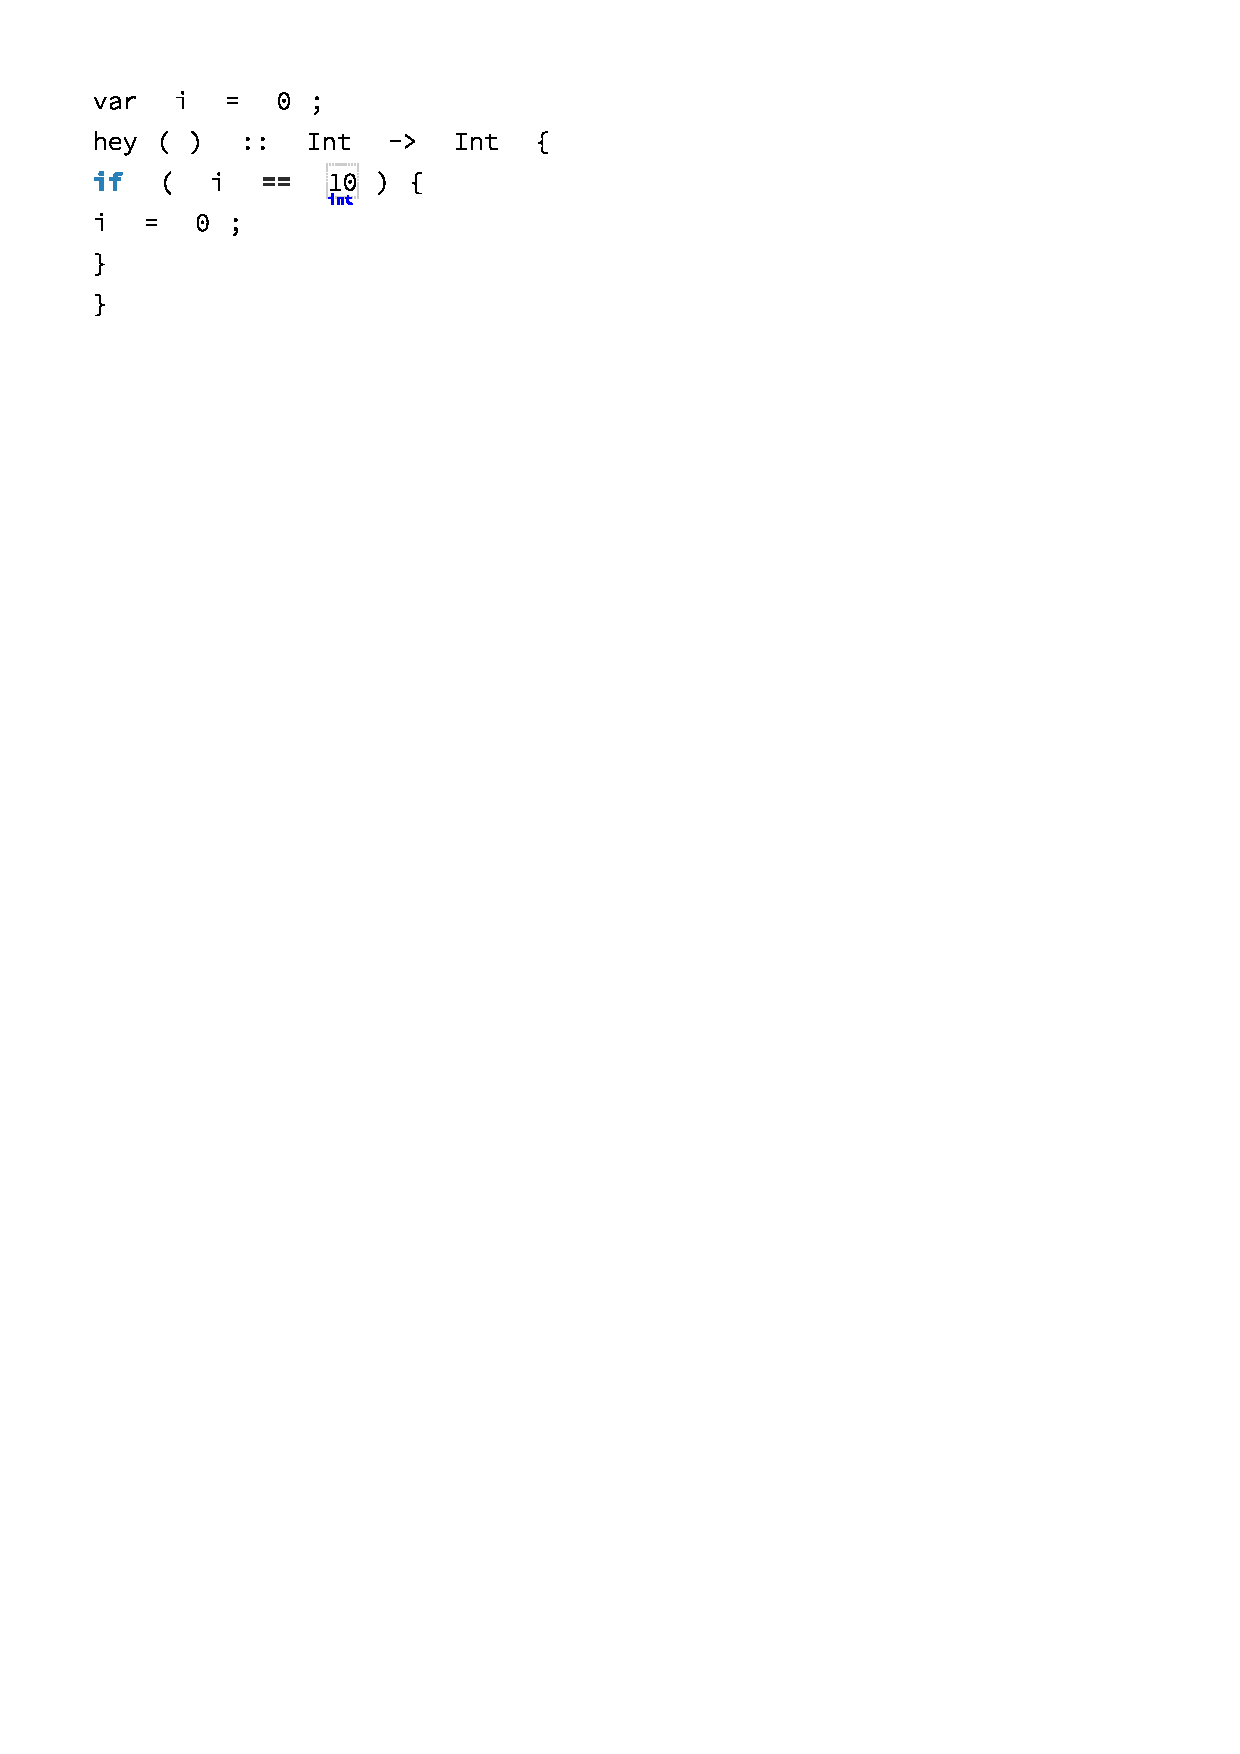
\includegraphics[width=6cm]{pics/lexer_html_debug.pdf}
				\end{minipage}%
		\subsection{Grammar}
			\paragraph{} As explained previously, I wanted to split parser and language. That's why I made a tiny parser for a tiny grammar description language. 
			\paragraph{Sublime text highlight definition} In order to work with the grammar confortably, I made a syntax definition for my favorite text editor, \href{https://www.sublimetext.com/}{Sublime Text}. You can find it in the tools directory.
			\subsubsection{Syntax}
				\paragraph{} Each line is a rule. A rule looks like that : \cc{Name~~~Step$_1$ Q$_1$, Step$_2$ Q$_2$, \dots, Step$_n$ Q$_n$}. The \cc{Step$_i$} will be described later. Indeed, a grammar rule consist of a series of tokens to match. \cc{Q$_1$} is optionnal; it can be \cc{+} (ie match this step one or more time) \cc{*} (ie match this step zero, one or more time), \cc{?} (match this step zero or one time).
				
				A \cc{Step} is of the form : \cc{Pattern$_1$ | Pattern$_2$ | \dots | Pattern$_m$}. A pattern is either a name (unquoted) of a rule, or a string refering to a \cc{TokenKind} (defined in one of the lexer's rules). A pattern can refer to a non yet existing rule. (circular references are then allowed - hopefully)


				\paragraph{Tree manipulation} You can use two modifier to perform basic tree manipulations: \cc{\#drop} and \cc{\#flattenIfNested}. 

				\cc{\#drop} operate on a node (let's denote it $A$) with only one child $B$: $A$ is remplaced by $B$. Indeed, sometimes, since this tiny grammar language is not very permissive, you need to split some rules to match some more complicated patterns: you don't really want that to be reflected in the AST. Then this drop modifier make that "artificial" node invisible.

				\cc{\#flattenIfNested} on a node $A$ will flatten children of $A$ whose type is $A$ also. If you match something using a direct recursive rule, then this modifier will turn a tree like $[a_1, [a_2, [a_3]]]$ into $[a_1, a_2, a_3]$ (where $a_i$ are nodes whose type is the same as $A$).

				\paragraph{} You can also provide a name for each step: for instance \cc{Step* as ident}. By naming each steps, it is easier to, later, manipulate the tree. Instead of saying "the first matched step", you say "the step named \textit{something}". This is particulary useful in the PrettyPrinter.

				\paragraph{} Check out the \cc{grammar.gr} provided for a more comprehensive view of the syntax and the possibilities.
			\subsubsection{Parser}
				The parser is very simple and very specific for this tiny language: we divide each lines, we filter comments, and we "consume" each steps. Each rules is "compiled" into a closure and registred (at first as an empty rule) into a cache, then after all rules compiled, we execute all closure. This allow recursive references over rules. The result is a JavaScript object (ie kind of a dictionnary) containing the main rule. \todo
			
		\subsection{Program generator}
			\paragraph{} After defining the grammar and the lexer rules, we know everything about what is a correct program for the parser. Then, in order to find some eventual buggy constructions, I decided to make a program generator.
			\paragraph{} By going through the grammar, we can generate a random program. If a step is mandatory, then no randomness is possible, but each time there is a modifier, we can apply some randomness. This way we build a sort of tree of the future program.
			
			The leafs are the token kind specified by the grammar. Theses token kinds are directly linked to regular expressions.  \href{https://fent.github.io/randexp.js/}{RandExp}, is a JavaScript library generating random strings matching a given regular expression. Using that library, I can generate any tokens.
			\paragraph{} The only issue is the size of the program generated: since it is random, I have no control over that. To solve that issue, I put some guardrail: after a certain (customizable) level of deepness, the algorithm try to stop as soon as possible to generate things (when the quantifier of a step is $*$ or $?$, we skip it; when it is $+$, we apply it only once).
			
			Also, after that limit, we avoid circular patterns used already as much as possible. For exemple, if we are in the expression $1 + 2 + 3 + 4$ (witch is in fact $\{1 + \{2 + \{3 + 4\}\}\}$ in the call stack), the circular rule managing the binary operators is used already 3 times, so we avoid it (if possible).

			The result is that the length of the generated program can explode but is still reasonnable, witch is what I wanted.

			\paragraph{State} I'm running this program generator for hours against my lexer and parser to see if there are some bugs. I spotted many errors (both due to grammar design and lexer/parser bugs), that I fixed. Now, it looks like it is ok.

			\paragraph{Issue} I introduced misformed error detection rules (i.e. avoiding ===), but that kinds of "excluding rules" are "bad": that can lead to inconsistencies and the program generator can't efficiently respect them. I think I will remove that from the lexer design.

			\paragraph{Issue} The generator do not take into account reserved words. Then, some errors can occurs. The solution 

		\subsection{Parser}
			\subsubsection{Optimization}
				\paragraph{} By analysing the grammar, I optimize the Parser: for each possible rule, we detect the possible starting lexems. Then, for any steps, we build a function that associate a lexem with a list of possibl rules. Then we avoid loads of recursion detections.

				Using this behaviour, the execution time was drastically reduced.

face\end{document}
